\subsection{Resize Rotates Entities}
Resizing an already rotated entity would result in an odd and unintuitive behaviour.
The problem was that the dragged vector just added its dimensions to the rectangles width and height.
However, if the rectangle is rotated, the dragged vector would still add its dimensions to the rectangle as if the rectangle was not rotated.
This issue would for example have a opposite resizing if the rectangle was rotated $90^\circ$, as can be seen in \figref{fig:resizeRotate}.
\begin{figure}[h]
	\centering
	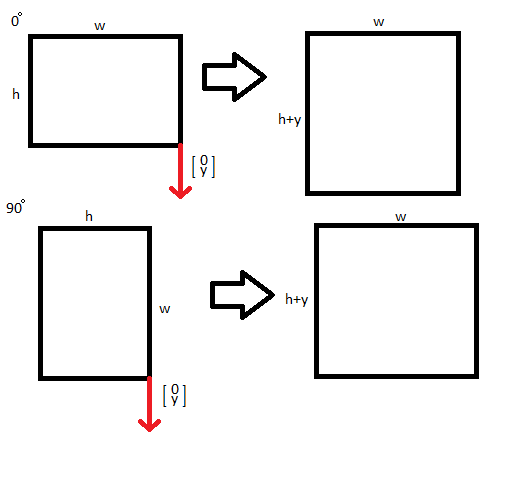
\includegraphics[scale=3]{media/sprint3/How-Rotate+Resize-Worked}
	\caption{Example showing previous resize rotate combination}
	\label{fig:resizeRotate}
\end{figure}
%Kan godt være den her linie skal skrives lidt om
To change this behaviour we tried some different ideas, which resulted in failure but will still be documented to show our effort towards this issue. 

%1: rotate then apply
The initial approach was to rotate the vector with the same angle as the rectangle is rotated and then apply the dimensions as previously.
However, this approach was mathematically flawed as the vector could end up with negative dimensions after rotation and decrease the size of the rectangle where the motion of the user intuitively should increase the size of the rectangle.

%2: rotate around a "pivot"
In an attempt to reuse the idea in the previous approach, we observe that the vector should be rotated somehow.
An example to show this idea can be shown using $\vec{a} =
\begin{bmatrix}
2 \\ 3
\end{bmatrix}$, and let us say the rectangle is rotated by $90^\circ$.
This means the resulting vector should be 
$\begin{bmatrix}
3 \\ 2
\end{bmatrix}$.
The problem with this approach is that we could not mathematically express how to rotate the vector.

%3: scale as much as hitbox grows
Since we can not determine that rotation, we take another approach and instead of looking at the drag vector, we look at how the hitbox changes. 
The drag vector was now applied to the hitbox and we looked at how much the hitbox would change in size.
This size change would then be applied to the rectangle inside the hitbox, but had the same problems as in the original problem as when the rectangle is rotated above $90^\circ$ its height should be changed when the hitbox width was changed.

%4: resize hitbox, keep smaller rect. properties/dimension
Next approach expanded upon the idea of using the hitbox. 
We look at where the edges of the rectangle connected with the hitbox and when the dimensions of the hitbox change, we place these edges at the same ratios.
For example, assume that the an edge of the rectangle connected with the side of a hitbox at a ratio of $20\% - 80\%$, it should keep that ratio after the hitbox is resized.
However, this approach will conceptually stretch the rectangle instead of resizing it, resulting in it no longer being a rectangle.
This result can not be represented with the implementation of the Android rectangle shape as the entity is considered a rectangle at all times, and due to this, it is not implemented.
\begin{figure}[h]
	\centering
	%---- linebreak	
	\begin{subfigure}[b]{0.45\textwidth}
		\centering
		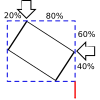
\includegraphics[scale=1.4]{media/sprint3/scaling-no-stretching}
		\caption{The rectangle without resizing.}
		\label{figure:app4.1}
	\end{subfigure}
	\qquad
	\begin{subfigure}[b]{0.45\textwidth}
		\centering
			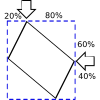
\includegraphics[scale=1.4]{media/sprint3/scaling-with-stretching}
			\caption{The rectangle after resizing.}
		\label{figure:app4.2}
	\end{subfigure}
	\caption{Example showing 4th resize approach.}
	\label{figure:app4}
\end{figure}
%5: width and height to vectors and resize acordingly.
Yet again we take the idea in another direction, and look at the width and height of the rectangle as vectors.
The angle of these vectors can be divided by the angle of the drag vector, to find a factor of how much each side has to be affected.
For example, let us assume that the width vector has an angle of $60^\circ$, the height vector an angle of $150^\circ$, and the drag vector $30^\circ$.
The factor can then be found as follows:
\begin{equation}
\begin{aligned}
w' &= v / w\\
h' &= 1 - w'\\
\end{aligned}
\end{equation}
where, 
\begin{itemize}
\item[$w$] is the angle of the width vector.
\item[$v$] is the angle of the drag vector.
\item[$w'$] is the factor of much the width should be affected.
\item[$h'$] is the factor of how much the height should be affected.
\end{itemize}
The equation is opposite when the angle of the width vector is above $90^\circ$.
With the above example the factors would be $w' = 0.5$ and $h' = 0.5$, which means half the length of the drag vector is added to the width and height.
A problem occurs when the angle of the width vector would be a lot smaller or larger than the drag vector angle and for example add twice the length of the drag vector.

%Current solution
The current and possibly final approach is to reset the starting point of the rectangle and swap its width and height.
This happens when the rotation angle of the rectangle is between $45^\circ$ and $315^\circ$, which corresponds to the possible angles to be between $45^\circ$ and $-45^\circ$.
We implement this approach since we observe that the resizing is reasonably accurate as long as the rotation angle is below $45^\circ$.
As an example, let the rotation of the rectangle be $46^\circ$, this means the dimensions of the rectangles are swapped and the rotation angle is set to $-44^\circ$, as can be seen in \figref{fig:app6}.
\begin{figure}
\centering
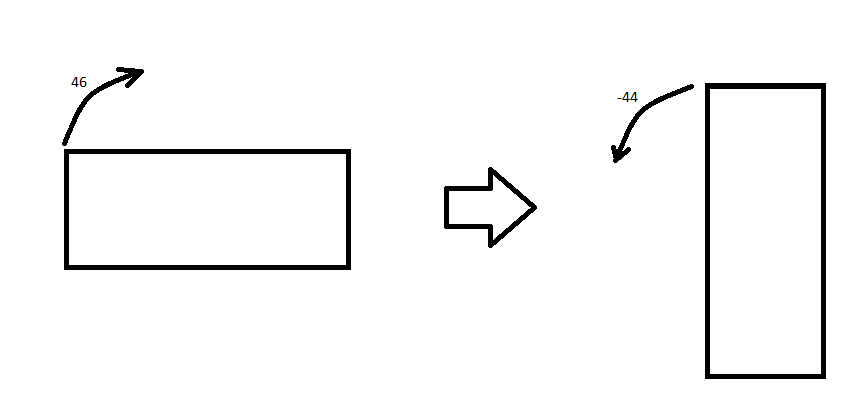
\includegraphics[scale=2]{media/sprint3/approach6}
\caption{Example showing the current and possibly final resize approach.}
\label{fig:app6}
\end{figure}
